\documentclass[border=4pt]{standalone}
\usepackage{tikz}
\usetikzlibrary{arrows.meta}

\definecolor{orangeText}{HTML}{E3A063}
\definecolor{orangeDim}{HTML}{A87A4E}
\begin{document}
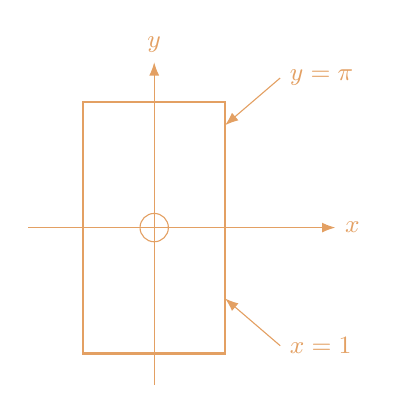
\begin{tikzpicture}[color=orangeText, >=Latex]

    % rectangle |x|<=1, |y|<=pi, with axes
    \draw[thick] (-0.9,-1.6) rectangle (0.9,1.6);
    \draw[->] (-1.6,0) -- (2.3,0) node[right] {\small $x$};
    \draw (0,-2.0) -- (0,1.6);
    \draw[->] (0,1.6) -- (0,2.1) node[above] {\small $y$};

    % small disc around the origin
    \draw (0,0) circle (0.18);

    \draw[<-] (0.9,1.3) -- (1.6,1.9) node[right] {\small $y=\pi$};
    \draw[<-] (0.9,-0.9) -- (1.6,-1.5) node[right] {\small $x=1$};

\end{tikzpicture}
\end{document}
